\cleardoublepage % memastikan bab baru dimulai di halaman ganjil (kanan)
\chapter{ANALISIS MASALAH}
\label{chap:analisis-masalah}

\section{Analisis Kondisi Saat Ini}
Sebelum mendefinisikan kebutuhan dan solusi pengembangan \textit{Warehouse Management Controller} (WMC), perlu dipahami terlebih dahulu kondisi operasional pergudangan PT Paragon Technology and Innovation saat ini beserta permasalahan yang melekat di dalamnya. Analisis kondisi saat ini dilakukan dengan menggali informasi langsung melalui wawancara dengan pihak Paragon Corp, menelaah proses bisnis \textit{warehouse} eksisting, serta mengidentifikasi kesenjangan (\textit{gap}) antara kondisi tersebut dengan target \textit{Smart Warehouse}. Seluruh analisis pada subbab ini bersumber dari hasil wawancara serta dokumen B100 subbab 2.1.3 Analisis Masalah \autocite{docB100}.

\subsection{Profil Operasional Gudang Berdasarkan Hasil Wawancara}
Guna memperoleh gambaran kondisi operasional yang akurat dan kontekstual, kelompok TA252601001 melaksanakan wawancara daring dengan Bapak Falih Muhtadi selaku \textit{Staff Logistics and Business Integration Systems} PT Paragon Technology and Innovation (Paragon Corp) pada tanggal 16 Oktober 2025. Dari wawancara tersebut diketahui bahwa Paragon Corp memiliki tiga jenis gudang, yaitu gudang bahan baku, gudang kemasan (\textit{packaging warehouse}), serta gudang barang jadi (\textit{Finished Goods}) yang terletak pada area terpisah. Fokus pengembangan tugas akhir ini adalah pada gudang barang jadi, yang secara langsung bersinggungan dengan proses distribusi produk ke konsumen akhir.

Berdasarkan hasil wawancara, sistem kerja operasional inventori Paragon Corp menerapkan pendekatan \textit{Pull System}, yaitu suatu mekanisme di mana pergerakan dan pemrosesan barang didasarkan pada permintaan aktual yang masuk ke sistem, bukan pada prakiraan (\textit{forecasting}) internal. Alur kerja utama gudang mencakup empat tahapan, yaitu \textit{Incoming}, \textit{Stocking}, \textit{Picking \& Checking}, serta \textit{Dispatching} menuju \textit{Distribution Center}. Dalam skema \textit{pull system}, perintah \textit{stocking} dan \textit{picking} baru dieksekusi ketika terdapat permintaan nyata, sehingga meminimalkan akumulasi stok berlebih (\textit{overstock}) namun di sisi lain menuntut kecepatan respons sistem yang sangat tinggi agar tidak menimbulkan \textit{bottleneck} pada tahap distribusi.

Dari hasil wawancara juga terungkap bahwa teknologi yang saat ini digunakan di gudang Paragon mencakup sistem ERP Odoo dan \textit{Warehouse Management System} (WMS) untuk pencatatan dan pelacakan barang. Namun, kedua sistem tersebut masih bersifat semi-manual sehingga membutuhkan input operator secara berkala dan belum memiliki integrasi \textit{real-time} antar platform. Kondisi ini menyebabkan \textit{mismatch} data yang sering terjadi antara kondisi fisik di lapangan dengan catatan digital pada sistem pusat. Paragon Corp sendiri saat ini tengah dalam proses transformasi menuju sistem SAP untuk meningkatkan kualitas integrasi antar sistem. Kompleksitas operasional semakin bertambah mengingat Paragon Corp mengelola lebih dari 40 \textit{Distribution Centers} (DC) di Indonesia dan Malaysia, dengan volume produk dan variasi SKU kosmetik yang sangat beragam, sehingga ketersediaan sistem inventori yang akurat dan terintegrasi menjadi kebutuhan operasional yang mendesak.

Wawancara tersebut turut mengonfirmasi permasalahan utama pada gudang barang jadi Paragon Corp, yang meliputi tiga hal: pertama, data stok tidak bersifat \textit{real-time} karena WMS belum terhubung langsung dengan sistem pusat; kedua, proses \textit{inbound} barang yang lambat dan perhitungan yang tidak presisi akibat ketergantungan pada proses manual; serta ketiga, proses \textit{picking} yang masih bergantung pada operator dan rawan \textit{human error}, khususnya dalam konteks jumlah barang. Bapak Falih juga mengonfirmasi adanya permasalahan \textit{mistracking} barang akibat area penempatan sementara yang tidak tercatat di sistem, serta potensi besar untuk mengotomasi proses \textit{inbound}, khususnya pemindahan barang dari truk ke \textit{pallet changer}.

\subsection{Proses Bisnis Pergudangan Eksisting}
Pada industri \textit{Fast Moving Consumer Goods} (FMCG) seperti PT Paragon Technology and Innovation, kebutuhan akan operasional rantai pasok menjadi kunci utama penggerak bisnis. Terdapat empat sumber daya utama yang menggerakkan sebuah \textit{warehouse}, yaitu \textit{storage system}, \textit{lift trucks}, \textit{personnel}, dan \textit{Warehouse Management System} (WMS). Kapasitas masing-masing komponen tersebut saling memengaruhi laju keseluruhan \textit{warehouse} sesuai prinsip \textit{flow impact test} (IFIT). Proses \textit{warehouse} secara umum mencakup: penerimaan (\textit{receiving}), penempatan (\textit{put-away}), pengisian ulang internal (\textit{internal replenishment}), pengambilan pesanan (\textit{order picking}), pengumpulan dan penyortiran (\textit{accumulating and sorting}), pengepakan (\textit{packing}), lintas-dermaga (\textit{cross docking}), pengiriman barang (\textit{dispatch}), dan pengapalan (\textit{shipping}).

Dari analisis proses operasional Paragon Corp yang termuat dalam dokumen B100, teridentifikasi sejumlah kelemahan mendasar pada kondisi eksisting. Pertama, sistem inventori disimpan secara independen dan tidak terintegrasi, sehingga berpotensi menimbulkan \textit{mismatch} data stok antara kondisi fisik dan catatan digital. Kedua, proses pencatatan dan pengambilan barang (\textit{case picking}) masih bergantung pada campur tangan operator manusia secara langsung. Hal ini menjadi hambatan operasional mengingat keterbatasan sumber daya manusia dalam hal kompetensi dan kuantitas merupakan salah satu kendala utama dalam proses \textit{picking} di industri \textit{warehousing}. Ketiga, walaupun Paragon Corp telah menggunakan robot \textit{Automated Guided Vehicle} (AGV) sebagai penunjang mobilisasi barang jadi, manajemen sistem armada AGV tersebut belum memiliki kerangka informasi yang jelas dan terintegrasi. Ketiga permasalahan ini secara kumulatif menciptakan tantangan operasional dalam konteks volume penyimpanan stok yang terus bertambah dan \textit{lead time} yang semakin ketat akibat tingginya permintaan industri FMCG.

Berdasarkan analisis proses bisnis \textit{Smart Warehouse} pada dokumen B100, disusun sejumlah aktivitas primer yang menjadi fokus optimasi sistem, sebagaimana dirangkum pada Tabel \ref{tab:aktivitas-primer}.

\begin{xltabular}{\textwidth}{ | l | X | }
  \caption{Aktivitas Primer pada \textit{Smart Warehouse}} \label{tab:aktivitas-primer} \\
  \hline
  \textbf{Kode} & \textbf{\textit{Activity}} \\
  \hline
  \endfirsthead
  \multicolumn{2}{l}{\textit{lanjutan Tabel \ref{tab:aktivitas-primer}}} \\
  \hline
  \textbf{Kode} & \textbf{\textit{Activity}} \\
  \hline
  \endhead
  \hline
  \endfoot
  PA01 & Otomatisasi Penerimaan Stok \\
  PA02 & Smart Storage \& Inventory \\
  PA03 & Order Picking and Warehouse Management Process \\
  PA04 & Quality Control \\
  PA05 & Smart Vendor Management \\
  PA06 & E-Procurement \& Smart Vendor Management \\
  \hline
\end{xltabular}

Fokus pengembangan \textit{Warehouse Management Controller} (WMC) pada tugas akhir ini diarahkan pada aktivitas PA01, PA02, dan PA03, sebagai aktivitas primer yang paling berkaitan dengan permasalahan otomasi penerimaan, penyimpanan, dan pengelolaan \textit{order} pada gudang Paragon Corp.

\subsection{Kondisi Sistem Saat Ini (As-Is)}
\label{sec:asis}
Pada kondisi saat ini, proses operasional gudang pada industri \textit{Fast Moving Consumer Goods} (FMCG) seperti Paragon Corp berjalan secara konvensional dengan mengandalkan tenaga kerja manusia dan proses manual di hampir seluruh tahapan. Alur proses keseluruhan pada kondisi eksisting digambarkan pada Gambar \ref{fig:bpmn-asis}.

\begin{figure}[h]
  \caption{Diagram BPMN proses bisnis \textit{warehouse} kondisi saat ini (\textit{As-Is})}
  \label{fig:bpmn-asis}
  \centering
  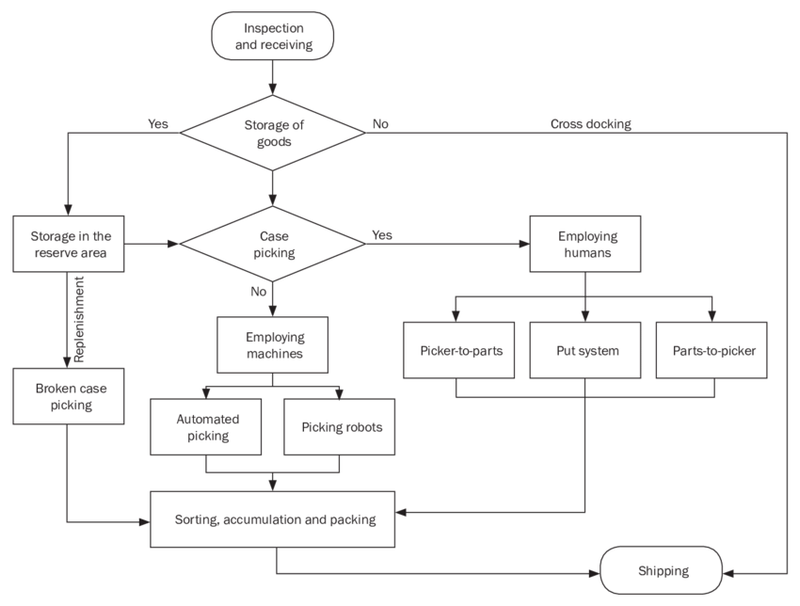
\includegraphics[width=\textwidth]{images/bpmn_asis.png}
\end{figure}

Proses diawali dengan tahap inspeksi dan penerimaan barang (\textit{inspection and receiving}), di mana staf gudang melakukan verifikasi fisik terhadap barang yang datang, mencakup pengecekan jumlah, kondisi kemasan, serta kesesuaiannya dengan dokumen pengiriman. Seluruh kegiatan pencatatan pada tahap ini masih dilakukan secara manual oleh staf gudang menggunakan dokumen fisik maupun lembar kerja yang tidak terintegrasi satu sama lain. Pendekatan ini rentan terhadap kesalahan pencatatan, ketidaksesuaian data antara dokumen fisik dan catatan digital, serta berpotensi memperlambat keseluruhan alur masuk barang apabila volume penerimaan terjadi dalam jumlah besar secara bersamaan. Tidak adanya mekanisme validasi otomatis pada tahap ini menjadikan keakuratan data penerimaan sepenuhnya bergantung pada ketelitian operator manusia.

Setelah barang berhasil diverifikasi, ditentukan apakah barang perlu disimpan terlebih dahulu ke area cadangan (\textit{storage of goods}) atau dapat langsung diteruskan melalui jalur \textit{cross docking}. Untuk barang yang memerlukan penyimpanan, staf secara manual menempatkan barang ke area penyimpanan cadangan (\textit{reserve area}). Selanjutnya, proses pengisian kembali (\textit{replenishment}) dilakukan untuk memastikan ketersediaan stok pada area aktif. Tidak adanya sistem pemantauan stok secara \textit{real-time} pada tahap ini menyebabkan proses \textit{replenishment} sering kali dilakukan berdasarkan estimasi visual operator di lapangan, sehingga berpotensi menimbulkan kondisi \textit{stockout} atau \textit{overstock} yang tidak terdeteksi secara cepat. Pada jalur \textit{cross docking}, barang yang tidak memerlukan penyimpanan langsung diteruskan ke tahap pengiriman, namun proses ini tetap bergantung pada koordinasi manual antara staf yang memperbesar risiko miskomunikasi dan keterlambatan.

Selanjutnya, sistem menentukan metode pengambilan barang (\textit{case picking}) yang akan digunakan. Apabila proses \textit{picking} dilakukan dengan melibatkan tenaga manusia (\textit{employing humans}), terdapat tiga metode yang dapat diterapkan, yaitu \textit{picker-to-parts} di mana operator bergerak menuju lokasi barang, \textit{put system} di mana barang dibawa ke stasiun sortir, dan \textit{parts-to-picker} di mana barang datang menuju operator. Keseluruhan metode ini masih bergantung sepenuhnya pada kinerja tenaga kerja manusia, sehingga kapasitas dan kecepatan operasional sangat dipengaruhi oleh kondisi fisik dan jumlah staf yang tersedia pada setiap waktu. Di sisi lain, apabila digunakan metode berbasis mesin (\textit{employing machines}), pilihan yang tersedia mencakup \textit{automated picking} dan \textit{picking robots}, namun kedua sistem ini beroperasi secara terpisah tanpa integrasi terpadu dengan sistem manajemen gudang, sehingga koordinasi antar subsistem masih memerlukan intervensi manual dari staf. Kondisi ini menciptakan \textit{bottleneck} operasional yang membatasi kapasitas pemenuhan pesanan, terutama pada periode permintaan tinggi.

Setelah proses \textit{picking} selesai, barang memasuki tahap sortir, akumulasi, dan pengemasan (\textit{sorting, accumulation, and packing}). Pada tahap ini, staf gudang memilah barang sesuai tujuan pengiriman, mengumpulkan barang per pesanan, dan mengemasnya secara manual untuk selanjutnya dikirimkan. Proses ini sangat bergantung pada ketelitian staf karena tidak terdapat sistem validasi otomatis yang memastikan kesesuaian barang yang dikemas dengan detail pesanan. Kondisi ini menyebabkan tingginya risiko kesalahan pengiriman (\textit{mispick}) yang baru terdeteksi pada tahap akhir distribusi, sehingga berpotensi menimbulkan pengembalian barang dan kerugian operasional. Setelah pengemasan selesai, barang dikirimkan (\textit{shipping}) kepada pelanggan atau distributor tujuan sebagai tahap akhir dari alur operasional gudang.

Secara keseluruhan, kondisi eksisting sistem pergudangan ini menunjukkan beberapa kelemahan struktural yang signifikan. Pertama, seluruh tahap operasional---mulai dari penerimaan, penyimpanan, \textit{picking}, hingga pengiriman---masih mengandalkan pencatatan dan koordinasi manual yang rentan terhadap kesalahan dan inkonsistensi data. Kedua, tidak adanya mekanisme pemantauan stok secara \textit{real-time} menyebabkan ketidaksinkronan yang berulang antara kondisi fisik di lapangan dan catatan digital pada sistem informasi. Ketiga, ketergantungan pada tenaga kerja manusia pada tahap \textit{picking} menciptakan \textit{bottleneck} operasional yang membatasi kapasitas dan kecepatan pemenuhan pesanan. Keempat, tidak adanya integrasi antar subsistem mengakibatkan visibilitas operasional yang terbatas bagi manajemen, sehingga memperlambat proses pengambilan keputusan serta meningkatkan potensi terjadinya \textit{human error} di setiap tahap operasional.

\subsection{Kondisi Sistem Smart Warehouse (To-Be)}
\label{sec:tobe}
Pada kondisi sistem \textit{Smart Warehouse} yang diusulkan, proses operasional gudang mengalami transformasi signifikan melalui penerapan \textit{Warehouse Management Controller} (WMC) yang mengintegrasikan antarmuka pengguna berbasis web, layanan manajemen pesanan, pengendalian armada robot, dan pembaruan inventori secara otomatis. Alur proses keseluruhan pada kondisi \textit{to-be} digambarkan pada Gambar \ref{fig:bpmn-tobe}.

\begin{figure}[h]
  \caption{Diagram BPMN proses bisnis \textit{Smart Warehouse} kondisi \textit{To-Be}}
  \label{fig:bpmn-tobe}
  \centering
  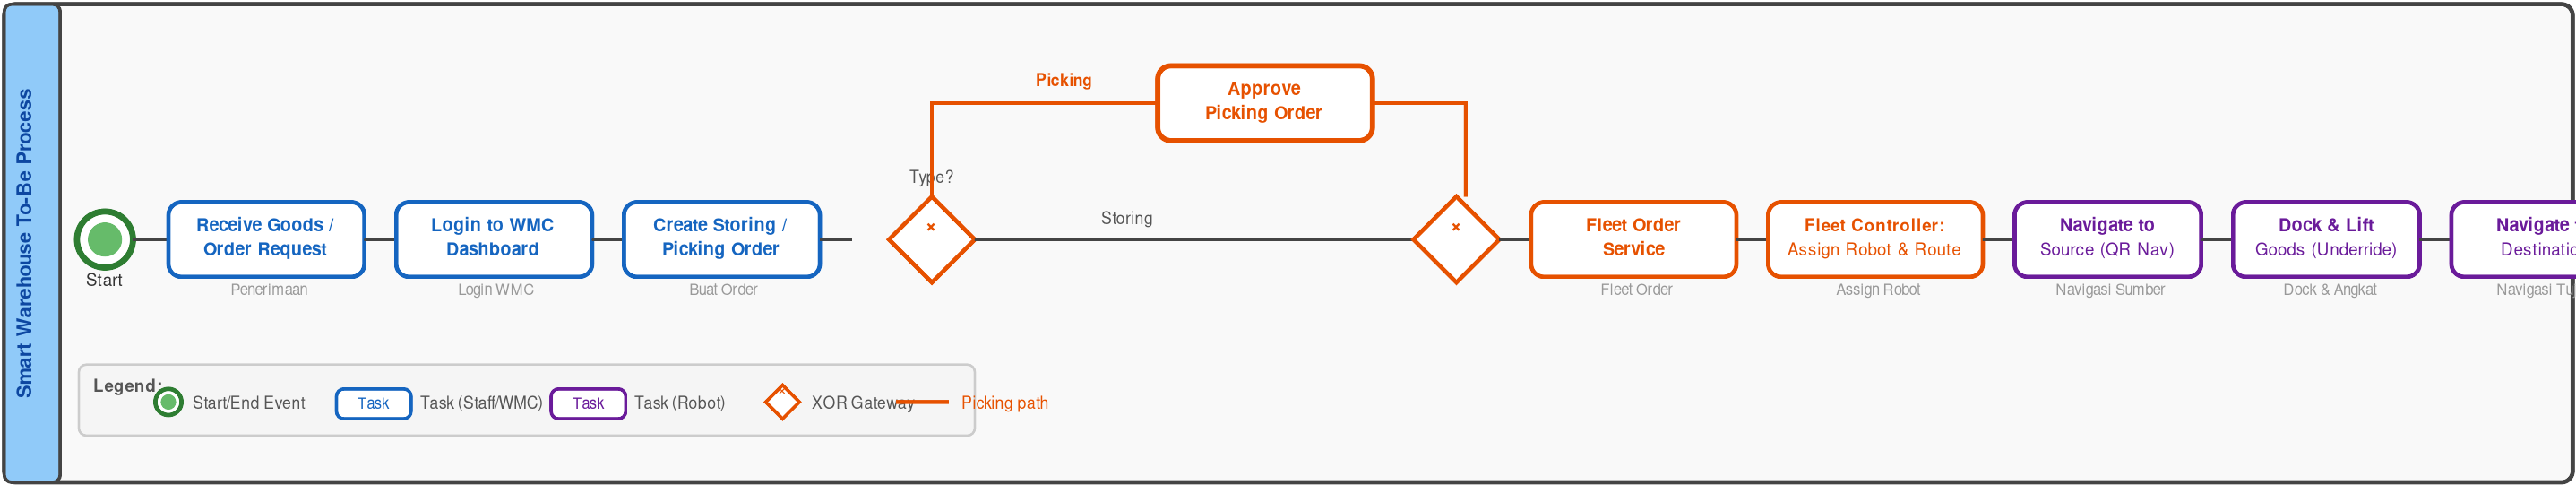
\includegraphics[width=\textwidth]{images/bpmn_tobe.png}
\end{figure}

Proses dimulai ketika staf gudang melakukan login ke dalam WMC \textit{Dashboard} melalui mekanisme autentikasi berbasis \textit{Bearer Token} yang diterbitkan oleh \textit{Authentication Service}. Setelah terautentikasi, staf membuat pesanan penyimpanan atau pengambilan barang (\textit{storing} atau \textit{picking}) melalui antarmuka WMC. Untuk pesanan \textit{picking}, diperlukan persetujuan dari manajer gudang sebelum pesanan diproses lebih lanjut, sehingga seluruh aktivitas pengambilan barang memiliki rekam jejak otorisasi yang terstruktur.

Pesanan yang telah disetujui diterima oleh \textit{Fleet Order Service} untuk divalidasi dan diteruskan ke \textit{Fleet Controller}. \textit{Fleet Controller} secara otomatis menentukan robot yang tersedia, mengalokasikan tugas, dan membangkitkan \textit{waypoint} rute pergerakan tanpa memerlukan intervensi manual dari staf. Seluruh proses penugasan ini berlangsung secara terpusat melalui sistem kendali yang terintegrasi.

Robot \textit{mobile} yang telah ditugaskan kemudian bergerak secara otonom menuju lokasi sumber barang menggunakan navigasi berbasis pemindaian \textit{QR code} dan sensor IMU. Sesampainya di lokasi, robot melakukan \textit{docking} dan mengangkat barang menggunakan mekanisme \textit{underride lifting}, kemudian bernavigasi menuju lokasi tujuan dan menurunkan barang secara presisi. Seluruh tahap pemindahan barang ini menggantikan proses \textit{picking} dan \textit{storing} manual yang sebelumnya dilakukan oleh tenaga kerja manusia.

Setelah robot menyelesaikan tugasnya, WMC secara otomatis memperbarui data inventori gudang melalui mekanisme \textit{event-driven} yang mencatat setiap perubahan stok sebagai \textit{event} diskrit. Status pesanan yang telah selesai langsung dikirimkan ke antarmuka WMC sehingga staf dapat memantau kondisi gudang secara \textit{real-time} tanpa perlu melakukan pencatatan manual, sehingga konsistensi antara kondisi fisik di lapangan dan data digital pada sistem selalu terjaga.

\subsection{Analisis Gap}
Dengan memahami kondisi eksisting \textit{warehouse} dan kondisi \textit{Smart Warehouse} yang ditargetkan, dilakukan analisis \textit{gap} untuk mengidentifikasi kesenjangan antara \textit{current condition} dan \textit{future condition} secara terstruktur. Analisis ini menjadi landasan utama dalam merumuskan kebutuhan sistem WMC. Tabel \ref{tab:gap-analysis} menyajikan hasil analisis \textit{gap} berdasarkan dokumen B100 Tabel 2.1.3.2.

\begin{xltabular}{\textwidth}{ | l | X | X | X | }
  \caption{\textit{Gap Analysis} Kondisi Eksisting vs \textit{Smart Warehouse} (B100 Tabel 2.1.3.2)} \label{tab:gap-analysis} \\
  \hline
  \textbf{Kode} & \textbf{Current Condition (Masalah Aktual Paragon)} & \textbf{Gap} & \textbf{Future Condition} \\
  \hline
  \endfirsthead
  \multicolumn{4}{l}{\textit{lanjutan Tabel \ref{tab:gap-analysis}}} \\
  \hline
  \textbf{Kode} & \textbf{Current Condition (Masalah Aktual Paragon)} & \textbf{Gap} & \textbf{Future Condition} \\
  \hline
  \endhead
  \hline
  \endfoot
  MA01 & Data stok tidak \textit{real-time}; WMS tidak terhubung dengan sistem pusat. & Tidak ada integrasi \textit{real-time} antar sistem (manual \textit{update}, rawan \textit{error}). & Sistem terintegrasi dan sinkron antara \textit{warehouse} barang jadi dan pusat. \\
  \hline
  MA02 & Pendataan dan penaruhan \textit{inbound} barang lambat; perhitungan barang tidak presisi. & Ketergantungan tinggi pada proses manual; \textit{error rate} tinggi dan proses lambat. & Sistem deteksi dan pelacakan barang akurat yang dilakukan secara otomatis. \\
  \hline
  MA03 & \textit{Picking} manual yang lambat dan ketergantungan dengan operator manusia. & Belum ada sistem otomasi untuk memastikan keakuratan permintaan dan waktu pemenuhan. & Sistem perpindahan barang dari semua tahapan dilakukan secara otomatis dan memenuhi keakuratan permintaan serta waktu. \\
  \hline
\end{xltabular}

Dari hasil analisis \textit{gap}, teridentifikasi tiga kelompok masalah aktual (MA01--MA03) yang secara langsung menjadi dasar perancangan WMC. Masalah MA01 berkaitan langsung dengan kebutuhan modul \textit{Goods Detail Service} untuk menjamin sinkronisasi stok \textit{real-time}; MA02 mendasari kebutuhan otomasi pencatatan dan pemantauan barang; sedangkan MA03 menjadi latar belakang pengembangan \textit{Fleet Order Service} untuk mengordinasikan armada robot dalam proses \textit{stocking} dan \textit{picking} secara terprogram.

\section{Analisis Kebutuhan}
Analisis kebutuhan bertujuan untuk mengidentifikasi secara sistematis dan menjabarkan seluruh persyaratan yang harus dipenuhi oleh \textit{Warehouse Management Controller} (WMC) guna menyelesaikan permasalahan operasional yang ada. Tahapan ini mencakup penjabaran karakteristik produk, penetapan kebutuhan fungsional dan nonfungsional, serta penjabaran batasan sistem sebagai landasan perancangan solusi yang tepat sasaran.

\subsection{Karakteristik Produk}
Berdasarkan tujuan proyek \textit{Smart Warehouse} yang telah dirumuskan pada dokumen B100 subbab 2.2.1, sistem \textit{Warehouse Management Controller} (WMC) dirancang untuk mengotomatisasi proses \textit{stocking} dan \textit{picking} pada pergudangan, mulai dari pencatatan, pelacakan, hingga perpindahan barang. Sistem ini memastikan integrasi data antara kondisi fisik dan digital secara \textit{real-time}, memungkinkan deteksi dan pemantauan pergerakan barang yang akurat, serta mendukung proses perpindahan barang secara presisi dan tepat waktu. Karakteristik produk tersebut dirangkum dan diberi kodefikasi pada Tabel \ref{tab:karakteristik-produk}.

\begin{xltabular}{\textwidth}{ | l | X | }
  \caption{Karakteristik Produk Sistem \textit{Smart Warehouse}} \label{tab:karakteristik-produk} \\
  \hline
  \textbf{Kode} & \textbf{Deskripsi} \\
  \hline
  \endfirsthead
  \multicolumn{2}{l}{\textit{lanjutan Tabel \ref{tab:karakteristik-produk}}} \\
  \hline
  \textbf{Kode} & \textbf{Deskripsi} \\
  \hline
  \endhead
  \hline
  \endfoot
  CH01 & Sistem dapat menyinkronkan data stok secara otomatis antara kondisi fisik dan catatan digital untuk menjaga konsistensi informasi inventori. \\
  \hline
  CH02 & Sistem mampu mendeteksi, mencatat, dan memantau pergerakan barang secara menyeluruh dari proses \textit{stocking} hingga \textit{picking}. \\
  \hline
  CH03 & Sistem dapat mengatur perpindahan barang secara otomatis dengan presisi sesuai waktu dan kebutuhan \textit{order}. \\
  \hline
  CH04 & Sistem menyajikan laporan \textit{real-time} kepada pengguna untuk mendukung pengambilan keputusan operasional. \\
  \hline
  CH05 & Sistem dapat menyesuaikan kapasitas dan alur kerja secara otomatis sesuai perubahan volume dan variasi produk. \\
  \hline
  CH06 & Sistem mampu beradaptasi dengan kebutuhan gudang yang berbeda melalui penyesuaian otomasi tambahan. \\
  \hline
  CH07 & Sistem mampu melakukan pembentukan \textit{order stocking} secara otomatis. \\
  \hline
\end{xltabular}

Karakteristik CH01--CH05 merupakan fungsi dasar yang menjadi inti kapabilitas sistem, sedangkan CH06--CH07 merupakan fungsi dan fitur tambahan. Ketujuh karakteristik produk ini menjadi acuan dalam penurunan kebutuhan fungsional dan nonfungsional WMC pada Subbab \ref{sec:kebutuhan-fungsional} dan \ref{sec:kebutuhan-nonfungsional} berikutnya.

\subsection{Kebutuhan Fungsional}
\label{sec:kebutuhan-fungsional}
Kebutuhan fungsional mendefinisikan kapabilitas spesifik yang harus dimiliki oleh \textit{Warehouse Management Controller} (WMC) untuk menyelesaikan setiap permasalahan yang telah diidentifikasi. Kebutuhan-kebutuhan berikut diturunkan dari karakteristik produk yang ditetapkan pada dokumen B100 (CH01--CH07) dan disesuaikan dengan lingkup pengembangan WMC sebagai sistem perangkat lunak yang mencakup \textit{Authentication Service}, \textit{Goods Detail Service}, \textit{Fleet Order Service}, dan \textit{User Interface}. Rincian kebutuhan fungsional disajikan pada Tabel \ref{tab:kebutuhan-fungsional}.

\begin{xltabular}{\textwidth}{ | l | X | l | }
  \caption{Kebutuhan Fungsional WMC} \label{tab:kebutuhan-fungsional} \\
  \hline
  \textbf{Kode} & \textbf{Deskripsi Kebutuhan} & \textbf{Acuan} \\
  \hline
  \endfirsthead
  \multicolumn{3}{l}{\textit{lanjutan Tabel \ref{tab:kebutuhan-fungsional}}} \\
  \hline
  \textbf{Kode} & \textbf{Deskripsi Kebutuhan} & \textbf{Acuan} \\
  \hline
  \endhead
  \hline
  \endfoot
  KF-01 & Login Pengguna --- Pengguna dapat melakukan login menggunakan \textit{username} dan \textit{password} yang terdaftar untuk mengakses fitur-fitur sistem WMC. & P-05 \\
  \hline
  KF-02 & Logout Pengguna --- Pengguna dapat melakukan \textit{logout} untuk mengakhiri sesi aktif dan keluar dari sistem WMC secara aman. & P-05 \\
  \hline
  KF-03 & Melihat Daftar Barang --- Pengguna dapat melihat daftar seluruh barang yang tersimpan di gudang beserta informasi ringkas seperti nama, SKU, kategori, dan jumlah stok. & CH01, P-01, P-02 \\
  \hline
  KF-04 & Melihat Detail Informasi Barang --- Pengguna dapat melihat informasi lengkap suatu barang, mencakup atribut, dimensi, berat, dan kondisi stok terkini. & CH01, P-01 \\
  \hline
  KF-05 & Melihat Lokasi Fisik Barang --- Pengguna dapat melihat lokasi penyimpanan fisik barang di dalam gudang, mencakup zona, rak, dan slot penyimpanan. & P-02 \\
  \hline
  KF-06 & Membuat Order Picking --- Pengguna dapat membuat \textit{order picking} untuk meminta robot mengambil barang dari lokasi penyimpanan ke titik keluaran gudang. & CH07, P-03 \\
  \hline
  KF-07 & Membuat Order Storing --- Pengguna dapat membuat \textit{order storing} untuk meminta robot menyimpan barang dari titik masuk ke lokasi penyimpanan yang sesuai. & CH03, P-03 \\
  \hline
  KF-08 & Melihat Daftar dan Status Order --- Pengguna dapat melihat seluruh daftar \textit{order} yang telah dibuat beserta status perkembangannya secara \textit{real-time}. & CH03, CH07, P-03 \\
  \hline
  KF-09 & Memantau Status Task Robot --- Pengguna dapat memantau status seluruh \textit{task} yang sedang maupun telah dieksekusi oleh robot, termasuk informasi kemajuan dan log aktivitas. & CH04, P-06 \\
  \hline
  KF-10 & Memantau Status Robot --- Pengguna dapat memantau kondisi operasional seluruh robot yang terdaftar dalam sistem, termasuk status, dan histori aktivitas robot. & CH04, P-06 \\
  \hline
\end{xltabular}

Selain kebutuhan fungsional pada lapisan WMC, pengembangan Subsistem Lokalisasi sebagai komponen pendukung \textit{Fleet Controller} juga memerlukan kebutuhan fungsional tersendiri, sebagaimana disajikan pada Tabel \ref{tab:kebutuhan-fungsional-lokalisasi}.

\begin{xltabular}{\textwidth}{ | l | X | l | }
  \caption{Kebutuhan Fungsional Subsistem Lokalisasi} \label{tab:kebutuhan-fungsional-lokalisasi} \\
  \hline
  \textbf{Kode} & \textbf{Deskripsi Kebutuhan} & \textbf{Acuan} \\
  \hline
  \endfirsthead
  \multicolumn{3}{l}{\textit{lanjutan Tabel \ref{tab:kebutuhan-fungsional-lokalisasi}}} \\
  \hline
  \textbf{Kode} & \textbf{Deskripsi Kebutuhan} & \textbf{Acuan} \\
  \hline
  \endhead
  \hline
  \endfoot
  KF-L01 & Mendeteksi dan Mengidentifikasi Objek --- Sistem dapat mendeteksi dan mengidentifikasi objek (robot, rak, \textit{docking station}) di area gudang menggunakan \textit{marker fiducial} unik. & B100/B300 -- Lokalisasi \\
  \hline
  KF-L02 & Pemetaan Posisi ke \textit{Grid} --- Sistem dapat memetakan posisi objek terdeteksi ke koordinat \textit{grid} diskrit sesuai \textit{layout} gudang. & B300 -- Representasi Posisi \\
  \hline
  KF-L03 & Penentuan Orientasi --- Sistem dapat menentukan orientasi (\textit{heading}) objek terdeteksi berbasis sudut pandang atas. & Paper Individu -- Klasifikasi \& Heading \\
  \hline
  KF-L04 & Publikasi Status Posisi --- Sistem dapat mempublikasikan status posisi terbaru secara berkala agar dikonsumsi \textit{Fleet Controller} dan \textit{Fleet Order Service} (WMC). & B200 -- Traceability \\
  \hline
\end{xltabular}

\subsection{Kebutuhan Nonfungsional}
\label{sec:kebutuhan-nonfungsional}
Kebutuhan nonfungsional mendefinisikan batasan kualitas dan performa yang harus dipenuhi oleh WMC sebagai atribut kualitas sistem di luar fungsi utamanya. Kebutuhan-kebutuhan ini diturunkan dari spesifikasi produk yang ditetapkan pada dokumen B200, khususnya pada aspek \textit{Usability}, \textit{Traceability}, \textit{Availability}, dan \textit{Safety} yang relevan dengan komponen perangkat lunak WMC. Rincian kebutuhan nonfungsional disajikan pada Tabel \ref{tab:kebutuhan-nonfungsional}.

\begin{longtable}{ | p{1.2cm} | p{1.8cm} | >{\raggedright\arraybackslash}p{4.7cm} | >{\raggedright\arraybackslash}p{2.1cm} | >{\raggedright\arraybackslash}p{2.1cm} | }
    \caption{Kebutuhan Nonfungsional WMC} \label{tab:kebutuhan-nonfungsional} \\
    \hline
    \textbf{Kode} & \textbf{Kategori} & \textbf{Deskripsi Kebutuhan} & \textbf{Parameter} & \textbf{Acuan} \\
    \hline
    \endfirsthead
    \multicolumn{5}{l}{\textit{lanjutan Tabel \ref{tab:kebutuhan-nonfungsional}}} \\
    \hline
    \textbf{Kode} & \textbf{Kategori} & \textbf{Deskripsi Kebutuhan} & \textbf{Parameter} & \textbf{Acuan} \\
    \hline
    \endhead
    \hline
    \endfoot
    KNF-01 & Usability & Sistem manajemen inventori dan \textit{fleet management} pada WMC harus memiliki tingkat kemudahan penggunaan yang tinggi sehingga mendukung pengambilan keputusan operasional secara cepat dan minim kesalahan oleh operator gudang. & SUS $>$ 80 & B200 -- Usability \\
    \hline
    KNF-02 & Traceability \& Latensi & Seluruh aktivitas pergerakan barang dan status robot harus tercatat secara lengkap dan berurutan tanpa kehilangan data, dengan sinkronisasi waktu antara robot--server dan server--WMS terjamin, serta pembaruan status robot dikirimkan ke server secara periodik. & Sinkronisasi $\leq$ 200 ms; status robot $\leq$ 1 detik & B200 -- Traceability \\
    \hline
    KNF-03 & Availability & Seluruh layanan WMC (\textit{Authentication Service}, \textit{Goods Detail Service}, \textit{Fleet Order Service}) harus dapat beroperasi secara kontinu selama jam operasional gudang tanpa \textit{downtime} yang tidak terencana, guna menjamin ketersediaan sistem bagi operator. & Availability $\geq$ 95\% & B200 -- Availability \\
    \hline
    KNF-04 & Keamanan & Seluruh \textit{endpoint} layanan WMC harus hanya dapat diakses oleh pengguna yang telah terautentikasi melalui mekanisme \textit{Bearer Token} yang diterbitkan oleh \textit{Authentication Service}, sehingga tidak ada akses tidak sah terhadap fungsi-fungsi kritis sistem. & 0 akses tanpa token valid & P-05, B200 -- Safety \\
    \hline
    KNF-05 & Konsistensi Data & Seluruh transaksi pengelolaan data inventori pada basis data terpusat WMC harus memenuhi properti ACID (\textit{Atomicity, Consistency, Isolation, Durability}) untuk menjamin tidak ada kondisi data yang setengah diperbarui atau inkonsisten antarlayanan meskipun terjadi kegagalan sistem. & 0 \textit{dirty read}; 0 \textit{partial update} & B200 -- Task Fulfilment Accuracy \\
    \hline
    KNF-06 & Skalabilitas & Arsitektur \textit{microservices} WMC harus memungkinkan setiap layanan (\textit{Authentication Service}, \textit{Goods Detail Service}, \textit{Fleet Order Service}) untuk dikembangkan, diuji, dan di-\textit{deploy} secara independen tanpa memerlukan \textit{redeployment} keseluruhan sistem, guna mendukung adaptasi terhadap kebutuhan gudang yang berbeda. & Independent deploy per service & CH05, CH06 \\
    \hline
\end{longtable}

Selain kebutuhan nonfungsional WMC, Subsistem Lokalisasi juga memiliki batasan kualitas dan performa tersendiri yang diturunkan dari dokumen B200, sebagaimana disajikan pada Tabel \ref{tab:kebutuhan-nonfungsional-lokalisasi}.

\begin{xltabular}{\textwidth}{ | p{1.6cm} | p{2.2cm} | X | p{2.6cm} | p{2.3cm} | }
  \caption{Kebutuhan Nonfungsional Subsistem Lokalisasi} \label{tab:kebutuhan-nonfungsional-lokalisasi} \\
  \hline
  \textbf{Kode} & \textbf{Kategori} & \textbf{Deskripsi Kebutuhan} & \textbf{Parameter} & \textbf{Acuan} \\
  \hline
  \endfirsthead
  \multicolumn{5}{l}{\textit{lanjutan Tabel \ref{tab:kebutuhan-nonfungsional-lokalisasi}}} \\
  \hline
  \textbf{Kode} & \textbf{Kategori} & \textbf{Deskripsi Kebutuhan} & \textbf{Parameter} & \textbf{Acuan} \\
  \hline
  \endhead
  \hline
  \endfoot
  KNF-L01 & Traceability \& Latensi & Status posisi robot diperbarui ke server dengan latensi tidak lebih dari 1 detik pada kondisi jaringan stabil. & Latensi $\leq$ 1 detik & B200 -- Traceability \\
  \hline
  KNF-L02 & Reliability & Sistem tidak mengalami degradasi akurasi posisi meskipun robot beroperasi berulang kali. & Task Repeatability 100\% & B200 -- Reliability \\
  \hline
  KNF-L03 & Availability \& Safety & Sistem dapat mendeteksi kegagalan pelacakan (\textit{mismatch} koordinat server vs posisi fisik) dan mengirimkan notifikasi yang memuat koordinat terakhir robot. & Notifikasi memuat \textit{last-known coordinate} & B200 -- Safety \\
  \hline
\end{xltabular}

\section{Analisis Pemilihan Solusi}
Berdasarkan identifikasi masalah dan kebutuhan yang telah dirumuskan pada sub-bab sebelumnya, tahap berikutnya adalah menganalisis dan menentukan solusi arsitektur yang paling sesuai untuk diimplementasikan sebagai \textit{Warehouse Management Controller} (WMC). Analisis ini dilakukan dengan terlebih dahulu mengidentifikasi alternatif-alternatif solusi yang mungkin, kemudian mengevaluasinya secara sistematis menggunakan metode \textit{Analytical Hierarchy Process} (AHP) sebagaimana yang telah ditetapkan pada dokumen B100, sehingga keputusan pemilihan solusi bersifat objektif dan dapat dipertanggungjawabkan secara teknis.

\subsection{Pemilihan Solusi Level WMC}

\subsubsection{Alternatif Solusi}
\label{sec:alternatif-solusi-wmc}
Dalam pengembangan WMC sebagai sistem perangkat lunak inti \textit{Smart Warehouse}, permasalahan utama yang perlu diselesaikan pada lapisan manajemen data adalah bagaimana sistem mencatat, memperbarui, dan menjaga konsistensi informasi inventori secara \textit{real-time} sejalan dengan aktivitas fisik robot di lapangan. Berdasarkan kajian pada dokumen B100 subbab 2.2.2.4, terdapat dua pendekatan arsitektur yang dapat dipertimbangkan sebagai solusi manajemen data inventori WMC, yaitu \textit{Event-Driven Inventory Management} dan \textit{State-Driven Inventory Management}. Karakteristik masing-masing alternatif diuraikan sebagai berikut.

\textbf{a. Alternatif 1: Event-Driven Inventory Management}

Pada pendekatan \textit{Event-Driven Inventory Management}, WMC mengelola \textit{order}, stok, dan proses pemindahan barang secara terintegrasi melalui mekanisme pencatatan \textit{event}. Ketika \textit{order stocking} atau \textit{picking} dibuat melalui \textit{Fleet Order Service}, sistem langsung mencatat \textit{order} dan melakukan reservasi stok secara internal untuk memastikan ketersediaan barang tanpa langsung mengurangi stok secara final. Setelah reservasi dilakukan, sistem mengirimkan instruksi pemindahan barang ke \textit{Fleet Controller}. Selama proses berlangsung, seluruh aktivitas dan hasil pemindahan dicatat sebagai \textit{event} operasional diskrit yang merepresentasikan kondisi fisik di lapangan. Berdasarkan hasil \textit{event} tersebut, sistem menentukan apakah pemindahan berhasil atau gagal, lalu memperbarui stok secara final atau mengembalikan stok ke kondisi semula sesuai hasil aktual.

Keunggulan utama alternatif ini terletak pada keseimbangan antara latensi rendah dan keandalan tinggi karena pembaruan stok hanya dilakukan setelah konfirmasi \textit{event} dari lapangan. Selain itu, riwayat seluruh pergerakan barang tetap tersimpan sebagai catatan \textit{event} yang dapat ditelusuri untuk kebutuhan audit dan analisis operasional, sehingga memenuhi persyaratan \textit{traceability} sesuai standar ISO 9001:2015. Adapun kekurangan dari pendekatan ini adalah kompleksitas implementasi yang lebih tinggi karena membutuhkan mekanisme pengelolaan \textit{event} yang terstruktur.

\textbf{b. Alternatif 2: State-Driven Inventory Management}

Pada pendekatan \textit{State-Driven Inventory Management}, WMC beroperasi dengan menjadikan satu sistem terpusat sebagai satu-satunya pengelola \textit{state} stok dan pergerakan barang. Ketika \textit{order picking} atau \textit{stocking} dibuat, sistem langsung mencatat \textit{order} dan sekaligus memperbarui stok secara langsung di basis data tanpa mekanisme reservasi bertingkat. Setelah \textit{order} tercatat, sistem mengirimkan instruksi ke \textit{Fleet Controller} untuk melakukan pemindahan barang. Apabila pemindahan gagal, sistem akan menyesuaikan kembali kondisi stok berdasarkan hasil aktual di lapangan. Setelah proses pemindahan selesai, data inventori terbaru disinkronisasi ke seluruh lapisan sistem sebagai referensi kondisi terkini.

Keunggulan utama alternatif ini adalah alur sistem yang lebih sederhana dengan kompleksitas implementasi yang lebih rendah dibandingkan pendekatan \textit{event-driven}, serta latensi yang rendah karena pembaruan stok dilakukan secara langsung. Proses pemantauan dan penelusuran masalah juga menjadi lebih mudah karena seluruh data \textit{state} terpusat di satu lokasi. Namun, kekurangan pendekatan ini adalah tingkat keandalan yang lebih rendah terhadap kegagalan parsial, karena jika terjadi kegagalan komunikasi antara WMC dan \textit{Fleet Controller} di tengah proses, konsistensi antara \textit{state} stok digital dan kondisi fisik barang tidak dapat dijamin secara otomatis. Selain itu, tidak adanya pencatatan \textit{event} membuat keterlacakan historis operasional menjadi terbatas.

\begin{xltabular}{\textwidth}{ | l | X | X | }
  \caption{Perbandingan Karakteristik Alternatif Solusi Manajemen Data Inventori} \label{tab:perbandingan-alternatif} \\
  \hline
  \textbf{Aspek} & \textbf{Alt. 1: Event-Driven} & \textbf{Alt. 2: State-Driven} \\
  \hline
  \endfirsthead
  \multicolumn{3}{l}{\textit{lanjutan Tabel \ref{tab:perbandingan-alternatif}}} \\
  \hline
  \textbf{Aspek} & \textbf{Alt. 1: Event-Driven} & \textbf{Alt. 2: State-Driven} \\
  \hline
  \endhead
  \hline
  \endfoot
  Mekanisme Pembaruan Stok & Bertahap: reservasi $\rightarrow$ eksekusi $\rightarrow$ konfirmasi \textit{event} $\rightarrow$ finalisasi stok & Langsung: pencatatan \textit{order} $\rightarrow$ pembaruan stok instan $\rightarrow$ eksekusi \\
  \hline
  Ketahanan terhadap Kegagalan Parsial & Tinggi --- stok hanya difinalisasi setelah konfirmasi hasil \textit{event} dari lapangan & Sedang --- risiko inkonsistensi stok jika kegagalan terjadi di tengah eksekusi \\
  \hline
  Keterlacakan (Traceability) & Komprehensif --- seluruh pergerakan barang tercatat sebagai \textit{event} historis yang dapat diaudit & Terbatas --- hanya mencatat \textit{state} akhir tanpa riwayat \textit{event} operasional \\
  \hline
  Kompleksitas Implementasi & Lebih tinggi --- membutuhkan mekanisme \textit{event handler}, reservasi, dan konfirmasi bertingkat & Lebih rendah --- alur sistem lebih sederhana dengan pembaruan langsung \\
  \hline
  Skalabilitas & Tinggi --- arsitektur \textit{loosely coupled} mendukung penambahan layanan tanpa perubahan besar & Sedang --- terpusat di satu \textit{state manager} sehingga \textit{scaling} lebih terbatas \\
  \hline
  Kemudahan Pemantauan & Sangat baik --- setiap \textit{event} tercatat sehingga diagnosis masalah dapat dilakukan secara mendetail & Mudah --- seluruh data terpusat di satu lokasi sehingga pemantauan sederhana \\
  \hline
  Skor AHP (B100) & 3,74 & 3,31 \\
  \hline
\end{xltabular}

\subsubsection{Analisis Penentuan Solusi}
Penentuan solusi dilakukan dengan mengevaluasi kedua alternatif yang telah diidentifikasi pada Subbab \ref{sec:alternatif-solusi-wmc} menggunakan metode \textit{Analytical Hierarchy Process} (AHP). Metode ini menghasilkan keputusan objektif dengan membandingkan setiap alternatif berdasarkan enam kriteria yang telah ditetapkan pada dokumen B100, yaitu \textit{Reliability}, \textit{Scalability}, \textit{Cost of Production}, \textit{Complexity of Production}, \textit{Task Completion Speed}, dan Kemudahan Penggunaan. Bobot setiap kriteria ditetapkan melalui proses perbandingan berpasangan dan telah divalidasi dengan nilai \textit{Consistency Ratio} (CR) yang memenuhi syarat konsistensi.

Bobot setiap kriteria yang digunakan sebagai dasar penilaian ditetapkan berdasarkan hasil perhitungan AHP pada dokumen B100. Nilai bobot mencerminkan tingkat kepentingan relatif setiap kriteria terhadap tujuan pemilihan solusi manajemen data inventori WMC, sebagaimana disajikan pada Tabel \ref{tab:bobot-ahp}.

\begin{xltabular}{\textwidth}{ | l | X | l | }
  \caption{Bobot Kriteria AHP Pemilihan Solusi Manajemen Data Inventori} \label{tab:bobot-ahp} \\
  \hline
  \textbf{Kriteria} & \textbf{Penjelasan} & \textbf{Bobot} \\
  \hline
  \endfirsthead
  \multicolumn{3}{l}{\textit{lanjutan Tabel \ref{tab:bobot-ahp}}} \\
  \hline
  \textbf{Kriteria} & \textbf{Penjelasan} & \textbf{Bobot} \\
  \hline
  \endhead
  \hline
  \endfoot
  Reliability & Ketahanan sistem bekerja secara konsisten dan akurat tanpa gangguan. & 0,36 \\
  \hline
  Scalability & Kemampuan sistem untuk dikembangkan sesuai peningkatan kebutuhan. & 0,25 \\
  \hline
  Cost of Production & Total biaya yang diperlukan untuk membuat dan mengoperasikan sistem. & 0,17 \\
  \hline
  Complexity of Production & Tingkat kesulitan dalam perancangan, pembuatan, dan integrasi sistem. & 0,11 \\
  \hline
  Task Completion Speed & Kecepatan sistem dalam menyelesaikan tugas permintaan dan penaruhan barang. & 0,07 \\
  \hline
  Kemudahan Penggunaan & Seberapa mudah sistem dioperasikan tanpa pelatihan khusus. & 0,05 \\
  \hline
\end{xltabular}

Berdasarkan bobot kriteria yang telah ditetapkan, setiap alternatif dievaluasi dengan memberikan nilai pada masing-masing kriteria sesuai karakteristik arsitekturnya. Tabel \ref{tab:penilaian-alt1} menyajikan penilaian dan justifikasi untuk Alternatif 1: \textit{Event-Driven Inventory Management}.

\begin{xltabular}{\textwidth}{ | l | c | X | }
  \caption{Penjelasan Penilaian Alternatif 1: Event-Driven Inventory Management} \label{tab:penilaian-alt1} \\
  \hline
  \textbf{Kriteria} & \textbf{Nilai} & \textbf{Penjelasan} \\
  \hline
  \endfirsthead
  \multicolumn{3}{l}{\textit{lanjutan Tabel \ref{tab:penilaian-alt1}}} \\
  \hline
  \textbf{Kriteria} & \textbf{Nilai} & \textbf{Penjelasan} \\
  \hline
  \endhead
  \hline
  \endfoot
  Reliability & 4 & Sistem memperbarui stok berdasarkan urutan kejadian (\textit{event}) sehingga data inventori tetap konsisten meskipun terjadi kegagalan pada robot di lapangan. \\
  \hline
  Scalability & 4 & Arsitektur berbasis \textit{event} memungkinkan sistem menangani peningkatan volume \textit{order} tanpa perubahan besar pada komponen inti layanan. \\
  \hline
  Cost of Production & 3 & Biaya pengembangan relatif moderat dan berskala linear sesuai kebutuhan tiap gudang. \\
  \hline
  Complexity of Production & 3 & Kompleksitas muncul pada perancangan mekanisme transisi status stok dan pengelolaan \textit{event handler} yang terstruktur. \\
  \hline
  Task Completion Speed & 3 & Proses penyelesaian tugas memerlukan waktu tambahan karena setiap perubahan stok harus melalui validasi kejadian (\textit{event confirmation}) terlebih dahulu. \\
  \hline
  Kemudahan Penggunaan & 5 & Pengguna lebih mudah mengoperasikan sistem karena seluruh data dan kontrol terpusat pada satu antarmuka terintegrasi. \\
  \hline
\end{xltabular}

Tabel \ref{tab:penilaian-alt2} menyajikan penilaian dan justifikasi untuk Alternatif 2: \textit{State-Driven Inventory Management}.

\begin{xltabular}{\textwidth}{ | l | c | X | }
  \caption{Penjelasan Penilaian Alternatif 2: State-Driven Inventory Management} \label{tab:penilaian-alt2} \\
  \hline
  \textbf{Kriteria} & \textbf{Nilai} & \textbf{Penjelasan} \\
  \hline
  \endfirsthead
  \multicolumn{3}{l}{\textit{lanjutan Tabel \ref{tab:penilaian-alt2}}} \\
  \hline
  \textbf{Kriteria} & \textbf{Nilai} & \textbf{Penjelasan} \\
  \hline
  \endhead
  \hline
  \endfoot
  Reliability & 3 & Keandalan sistem bergantung pada satu pusat pengelolaan \textit{state} sehingga operasi tetap stabil selama sistem utama berjalan, namun berisiko inkonsistensi stok jika terjadi kegagalan di tengah eksekusi. \\
  \hline
  Scalability & 3 & Peningkatan kapasitas sistem memerlukan penambahan sumber daya pada sistem pusat, sehingga \textit{scaling} lebih terbatas dibandingkan pendekatan berbasis \textit{event}. \\
  \hline
  Cost of Production & 3 & Biaya produksi berada pada tingkat menengah karena sistem terpusat membutuhkan infrastruktur yang cukup andal. \\
  \hline
  Complexity of Production & 4 & Kompleksitas pengembangan lebih rendah karena seluruh logika inventori dan pemindahan barang berada dalam satu sistem yang terpusat. \\
  \hline
  Task Completion Speed & 4 & Penyelesaian tugas berlangsung cepat karena keputusan dan pembaruan stok dilakukan langsung tanpa proses sinkronisasi \textit{event} bertingkat. \\
  \hline
  Kemudahan Penggunaan & 5 & Pengguna lebih mudah mengoperasikan sistem karena seluruh data dan kontrol terpusat pada satu antarmuka. \\
  \hline
\end{xltabular}

Setelah seluruh kriteria dinilai untuk kedua alternatif, skor akhir diperoleh dengan mengalikan nilai setiap kriteria dengan bobot yang telah ditetapkan, lalu dijumlahkan. Rekapitulasi perhitungan AHP disajikan pada Tabel \ref{tab:rekap-ahp}.

\begin{xltabular}{\textwidth}{ | X | c | c | c | c | c | }
  \caption{Rekapitulasi Penilaian AHP Solusi Manajemen Data Inventori (B100 Tabel 2.2.3.8)} \label{tab:rekap-ahp} \\
  \hline
  \multirow{2}{*}{\textbf{Kriteria}} & \multirow{2}{*}{\textbf{Bobot}} & \multicolumn{2}{c|}{\textbf{Alt. 1: Event-Driven}} & \multicolumn{2}{c|}{\textbf{Alt. 2: State-Driven}} \\
  \cline{3-6}
   & & \textbf{Nilai} & \textbf{Bobot$\times$Nilai} & \textbf{Nilai} & \textbf{Bobot$\times$Nilai} \\
  \hline
  \endfirsthead
  \multicolumn{6}{l}{\textit{lanjutan Tabel \ref{tab:rekap-ahp}}} \\
  \hline
  \multirow{2}{*}{\textbf{Kriteria}} & \multirow{2}{*}{\textbf{Bobot}} & \multicolumn{2}{c|}{\textbf{Alt. 1: Event-Driven}} & \multicolumn{2}{c|}{\textbf{Alt. 2: State-Driven}} \\
  \cline{3-6}
   & & \textbf{Nilai} & \textbf{Bobot$\times$Nilai} & \textbf{Nilai} & \textbf{Bobot$\times$Nilai} \\
  \hline
  \endhead
  \hline
  \endfoot
  Reliability & 0,36 & 4 & 1,44 & 3 & 1,08 \\
  \hline
  Scalability & 0,25 & 4 & 1,00 & 3 & 0,75 \\
  \hline
  Cost of Production & 0,17 & 3 & 0,51 & 3 & 0,51 \\
  \hline
  Complexity of Prod. & 0,11 & 3 & 0,33 & 4 & 0,44 \\
  \hline
  Task Completion Speed & 0,07 & 3 & 0,21 & 4 & 0,28 \\
  \hline
  Kemudahan Penggunaan & 0,05 & 5 & 0,25 & 5 & 0,25 \\
  \hline
  \textbf{Total} & \textbf{1} & --- & \textbf{3,74} & --- & \textbf{3,31} \\
  \hline
\end{xltabular}

Berdasarkan hasil perhitungan AHP pada Tabel \ref{tab:rekap-ahp}, Alternatif 1: \textit{Event-Driven Inventory Management} memperoleh skor total 3,74, lebih tinggi dibandingkan Alternatif 2: \textit{State-Driven Inventory Management} dengan skor 3,31. Keunggulan utama \textit{Event-Driven} terletak pada aspek \textit{Reliability} (bobot tertinggi 0,36) dan \textit{Scalability} (0,25) yang secara agregat memberikan kontribusi skor lebih besar, mencerminkan kemampuan arsitektur berbasis \textit{event} dalam menjaga konsistensi data stok meskipun terjadi kegagalan pada komponen fisik robot, serta fleksibilitasnya dalam menangani peningkatan volume transaksi tanpa membebani satu titik pusat sistem.

Dengan demikian, berdasarkan analisis AHP tersebut, \textit{Event-Driven Inventory Management} dipilih sebagai arsitektur solusi yang diimplementasikan pada \textit{Warehouse Management Controller} (WMC) dalam tugas akhir ini. Keputusan ini selaras dengan kesimpulan pada dokumen B100 subbab 2.2.4, di mana \textit{Event-Driven Inventory Management} ditetapkan sebagai solusi manajemen inventori terpilih karena kemampuannya menjaga konsistensi data stok melalui pencatatan setiap perubahan sebagai \textit{event}, serta memudahkan proses audit dan keterlacakan operasional gudang.

\subsection{Pemilihan Solusi Subsistem Lokalisasi}
Selain solusi arsitektur WMC pada Subbab \ref{sec:alternatif-solusi-wmc}, subbab ini menjabarkan pemilihan solusi teknis untuk subsistem lokalisasi menggunakan metode \textit{Analytical Hierarchy Process} (AHP) yang sama, guna menjustifikasi pemilihan AprilTag dan kamera \textit{fisheye overhead} dibandingkan alternatif lain.

\subsubsection{Alternatif Solusi Lokalisasi}
Sama seperti pada subbab sebelumnya, pemilihan solusi teknis untuk subsistem lokalisasi diawali dengan mengidentifikasi alternatif pendekatan lokalisasi yang dapat diterapkan. Berdasarkan kajian pada dokumen B100/B300 dan implementasi yang dilakukan pada tugas akhir ini, terdapat dua pendekatan yang dapat dipertimbangkan, yaitu \textit{QR Code + Line Following} dan \textit{AprilTag + Overhead Fisheye Camera}. Karakteristik masing-masing alternatif diuraikan sebagai berikut.

\textbf{a. Alternatif 1: QR Code + Line Following}

Pendekatan ini menempatkan seluruh perangkat lokalisasi pada masing-masing robot (\textit{on-board}, desentralisasi) sebagaimana dirancang pada dokumen B100/B300. Robot mengikuti garis lintasan di lantai secara kontinu menggunakan \textit{Line Detector Sensor} BFD-1000 (6 kanal IR) untuk memperoleh posisi relatif terhadap jalur, kemudian memindai \textit{QR code} menggunakan GM65 \textit{reader} pada titik-titik tertentu untuk memverifikasi posisi absolut dalam matriks \textit{grid} $12\times6$. Data ini digabung dengan pembacaan IMU dan diolah oleh ESP32-S3 di tiap robot untuk menghasilkan status posisi yang dikirim ke \textit{Fleet Controller}.

Keunggulan utama alternatif ini adalah setiap robot mandiri melakukan \textit{self-localization} sehingga tidak bergantung pada satu titik kegagalan sentral, dan infrastruktur jalur serta \textit{QR code} relatif murah untuk dipasang di lantai gudang. Adapun kekurangannya, akurasi posisi antar-\textit{checkpoint} bergantung pada kestabilan pembacaan sensor garis yang sensitif terhadap kondisi lantai (debu, aus, pencahayaan), setiap robot memerlukan satu set sensor lengkap sehingga biaya bertambah linear seiring penambahan robot, dan verifikasi posisi absolut hanya terjadi secara diskrit di titik \textit{QR}, bukan kontinu di seluruh area.

\textbf{b. Alternatif 2: AprilTag + Overhead Fisheye Camera}

Pendekatan ini memindahkan seluruh proses lokalisasi ke satu titik sentral, yaitu kamera IP \textit{fisheye} 1080p yang dipasang setinggi 60 cm di atas area lantai gudang ($2,4\times1,2$ m), melakukan \textit{streaming} video melalui protokol RTSP, kemudian diproses oleh Subsistem Lokalisasi di server melalui \textit{pipeline} koreksi distorsi Kannala--Brandt $\rightarrow$ transformasi \textit{homography} $\rightarrow$ deteksi \textit{marker} AprilTag Tag36h11 $\rightarrow$ \textit{snapping} ke sel \textit{grid}, yang berjalan pada frekuensi 4 Hz dan dipublikasikan ke \textit{topic} MQTT \texttt{location} setiap 500 ms. Pendekatan inilah yang diimplementasikan pada tugas akhir ini.

Keunggulan utama alternatif ini adalah satu perangkat mampu mencakup seluruh area tanpa oklusi, akurasi terverifikasi 100\% pada pengujian posisi maupun orientasi (Tabel \ref{tab:verifikasi-posisi}--\ref{tab:verifikasi-orientasi}), kalibrasi \textit{homography} hanya dilakukan sekali di awal pemasangan (\textit{one-time}), dan penambahan robot baru cukup dilakukan dengan menempelkan \textit{marker} AprilTag baru tanpa tambahan sensor per unit. Adapun kekurangannya, pendekatan ini bersifat \textit{single point of failure} karena jika kamera atau koneksi RTSP mengalami gangguan maka seluruh sistem lokalisasi ikut lumpuh, area cakupan dibatasi oleh \textit{field-of-view} satu kamera sehingga perluasan ke gudang yang lebih besar memerlukan penambahan kamera dan proses \textit{stitching}, serta memerlukan tahap kalibrasi optik yang lebih matematis dibandingkan sensor garis.

\begin{xltabular}{\textwidth}{ | l | X | X | }
  \caption{Perbandingan Karakteristik Alternatif Solusi Lokalisasi} \label{tab:perbandingan-alternatif-lokalisasi} \\
  \hline
  \textbf{Aspek} & \textbf{Alt. 1: QR Code + Line Following} & \textbf{Alt. 2: AprilTag + Overhead Fisheye} \\
  \hline
  \endfirsthead
  \multicolumn{3}{l}{\textit{lanjutan Tabel \ref{tab:perbandingan-alternatif-lokalisasi}}} \\
  \hline
  \textbf{Aspek} & \textbf{Alt. 1: QR Code + Line Following} & \textbf{Alt. 2: AprilTag + Overhead Fisheye} \\
  \hline
  \endhead
  \hline
  \endfoot
  Arsitektur Pemrosesan & Desentralisasi --- tiap robot (ESP32-S3) mengolah posisinya sendiri & Sentralisasi --- satu server mengolah seluruh objek dari satu kamera \\
  \hline
  Sumber Posisi Absolut & \textit{QR code}, dibaca diskrit di titik tertentu & AprilTag, terdeteksi kontinu di setiap \textit{frame} (4 Hz) \\
  \hline
  Cakupan Area & Seluruh lantai (jalur + titik QR tersebar) & Dibatasi \textit{field-of-view} satu kamera per titik pemasangan \\
  \hline
  Akurasi Terukur & Tidak diuji langsung pada TA ini (target \textit{repeatability} 100\% di B200) & 100\% pada 6 kasus posisi \& 4 kasus orientasi (Tabel \ref{tab:verifikasi-posisi}--\ref{tab:verifikasi-orientasi}) \\
  \hline
  Latensi Publikasi & Target $\leq$1 detik (KNF-L01) & Terukur 500 ms \\
  \hline
  Penambahan Robot Baru & Perlu sensor lengkap (BFD-1000, GM65, IMU, ESP32-S3) per unit & Cukup \textit{marker} AprilTag cetak per unit \\
  \hline
  Titik Kegagalan & Terdistribusi per robot & Terpusat pada satu kamera/server \\
  \hline
  Sensitivitas Lingkungan & Aus/kotor pada garis \& \textit{marker} lantai & Pencahayaan \& oklusi terhadap kamera \\
  \hline
\end{xltabular}

\subsubsection{Kriteria Evaluasi}
Berbeda dengan pemilihan solusi level WMC yang menggunakan kembali kriteria umum dari dokumen B100, pemilihan solusi lokalisasi memerlukan kriteria yang lebih spesifik terhadap karakteristik teknis lokalisasi robot. Kriteria evaluasi ditetapkan berdasarkan keterkaitannya dengan kebutuhan nonfungsional subsistem lokalisasi (KNF-L01--KNF-L03) pada Tabel \ref{tab:kebutuhan-nonfungsional-lokalisasi}, mencakup aspek akurasi, latensi, skalabilitas, ketahanan operasional, biaya, dan kompleksitas kalibrasi, sebagaimana dirangkum pada Tabel \ref{tab:kriteria-evaluasi-lokalisasi}.

\begin{xltabular}{\textwidth}{ | l | X | }
  \caption{Kriteria Evaluasi Pemilihan Solusi Lokalisasi} \label{tab:kriteria-evaluasi-lokalisasi} \\
  \hline
  \textbf{Kriteria} & \textbf{Penjelasan} \\
  \hline
  \endfirsthead
  \multicolumn{2}{l}{\textit{lanjutan Tabel \ref{tab:kriteria-evaluasi-lokalisasi}}} \\
  \hline
  \textbf{Kriteria} & \textbf{Penjelasan} \\
  \hline
  \endhead
  \hline
  \endfoot
  Akurasi Posisi & Ketepatan sistem memetakan posisi fisik robot ke koordinat \textit{grid} dan orientasi (\textit{heading}) sebenarnya. \\
  \hline
  Latensi Publikasi & Kecepatan sistem memperbarui status posisi ke server/UI sejak perubahan posisi fisik terjadi. \\
  \hline
  Skalabilitas ke Banyak Robot & Kemudahan dan biaya marjinal menambah robot baru ke dalam sistem lokalisasi. \\
  \hline
  Ketahanan Operasional (Reliability) & Konsistensi akurasi sistem terhadap kondisi lingkungan (pencahayaan, kotoran, aus) dan operasi berulang, terkait KNF-L02. \\
  \hline
  Biaya Implementasi & Total biaya perangkat keras yang dibutuhkan untuk mencakup seluruh area dan armada robot. \\
  \hline
  Kompleksitas Kalibrasi & Tingkat kesulitan proses instalasi dan kalibrasi awal sebelum sistem dapat digunakan. \\
  \hline
\end{xltabular}

\subsubsection{Pairwise Comparison dan Perhitungan Bobot Kriteria}
Penentuan bobot kriteria dilakukan melalui metode \textit{Analytical Hierarchy Process} (AHP) dengan melakukan perbandingan berpasangan (\textit{pairwise comparison}) antar keenam kriteria pada Tabel \ref{tab:kriteria-evaluasi-lokalisasi}. Urutan kepentingan kriteria ditetapkan berdasarkan keterkaitannya dengan kebutuhan nonfungsional inti subsistem lokalisasi: Akurasi Posisi dan Latensi Publikasi diprioritaskan karena berkaitan langsung dengan pemenuhan KNF-L01 dan KNF-L02, diikuti oleh Skalabilitas, Ketahanan Operasional, Biaya Implementasi, dan Kompleksitas Kalibrasi. Hasil perbandingan berpasangan menggunakan skala Saaty disajikan pada Tabel \ref{tab:pairwise-lokalisasi} (kriteria disingkat berturut-turut sebagai AP, LP, SK, KO, BI, dan KK sesuai urutan pada Tabel \ref{tab:kriteria-evaluasi-lokalisasi}).

{\small
\begin{xltabular}{\textwidth}{ | X | c | c | c | c | c | c | }
  \caption{Nilai Kepentingan Kriteria} \label{tab:pairwise-lokalisasi} \\
  \hline
  \textbf{Kriteria} & \textbf{AP} & \textbf{LP} & \textbf{SK} & \textbf{KO} & \textbf{BI} & \textbf{KK} \\
  \hline
  \endfirsthead
  \multicolumn{7}{l}{\textit{lanjutan Tabel \ref{tab:pairwise-lokalisasi}}} \\
  \hline
  \textbf{Kriteria} & \textbf{AP} & \textbf{LP} & \textbf{SK} & \textbf{KO} & \textbf{BI} & \textbf{KK} \\
  \hline
  \endhead
  \hline
  \endfoot
  Akurasi Posisi (AP) & 1 & 2 & 3 & 4 & 4 & 4 \\
  \hline
  Latensi Publikasi (LP) & 0,5 & 1 & 2 & 3 & 4 & 4 \\
  \hline
  Skalabilitas (SK) & 0,33 & 0,5 & 1 & 2 & 3 & 4 \\
  \hline
  Ketahanan Operasional (KO) & 0,25 & 0,33 & 0,5 & 1 & 2 & 3 \\
  \hline
  Biaya Implementasi (BI) & 0,25 & 0,25 & 0,33 & 0,5 & 1 & 2 \\
  \hline
  Kompleksitas Kalibrasi (KK) & 0,25 & 0,25 & 0,25 & 0,33 & 0,5 & 1 \\
  \hline
\end{xltabular}
}

Bobot masing-masing kriteria dihitung dengan menormalisasi setiap kolom matriks terhadap jumlah kolomnya, kemudian merata-ratakan nilai pada setiap baris (metode \textit{eigenvector} approksimasi), sebagaimana dilakukan pada dokumen B100. Hasil perhitungan bobot disajikan pada Tabel \ref{tab:bobot-ahp-lokalisasi}.

\begin{xltabular}{\textwidth}{ | X | c | }
  \caption{Nilai Bobot Kriteria} \label{tab:bobot-ahp-lokalisasi} \\
  \hline
  \textbf{Kriteria} & \textbf{Bobot} \\
  \hline
  \endfirsthead
  \multicolumn{2}{l}{\textit{lanjutan Tabel \ref{tab:bobot-ahp-lokalisasi}}} \\
  \hline
  \textbf{Kriteria} & \textbf{Bobot} \\
  \hline
  \endhead
  \hline
  \endfoot
  Akurasi Posisi & 0,36 \\
  \hline
  Latensi Publikasi & 0,25 \\
  \hline
  Skalabilitas ke Banyak Robot & 0,17 \\
  \hline
  Ketahanan Operasional (Reliability) & 0,11 \\
  \hline
  Biaya Implementasi & 0,07 \\
  \hline
  Kompleksitas Kalibrasi & 0,05 \\
  \hline
  \textbf{Total} & \textbf{1,00} \\
  \hline
\end{xltabular}

Uji konsistensi terhadap matriks perbandingan berpasangan pada Tabel \ref{tab:pairwise-lokalisasi} menghasilkan nilai \textit{eigenvalue} maksimum ($\lambda_{maks}$) sebesar 6,226. \textit{Consistency Index} (CI) dihitung dengan rumus $CI = (\lambda_{maks} - n)/(n-1) = (6,226-6)/(6-1) = 0,045$. Dengan nilai \textit{Random Index} (RI) untuk matriks berukuran $n=6$ sebesar 1,24 \autocite{saaty1977}, diperoleh \textit{Consistency Ratio} $CR = CI/RI = 0,045/1,24 = 0,036$. Karena $CR = 0,036 < 0,1$, matriks perbandingan berpasangan pada Tabel \ref{tab:pairwise-lokalisasi} dinyatakan konsisten sehingga bobot kriteria pada Tabel \ref{tab:bobot-ahp-lokalisasi} dapat digunakan sebagai dasar penilaian alternatif.

\subsubsection{Penilaian Alternatif dan Penentuan Solusi Terpilih}
\label{sec:penilaian-alternatif-lokalisasi}
Berdasarkan bobot kriteria yang telah ditetapkan pada Tabel \ref{tab:bobot-ahp-lokalisasi}, setiap alternatif dievaluasi dengan memberikan nilai pada skala 1--5 (1 = sangat buruk, 5 = sangat baik) untuk masing-masing kriteria sesuai karakteristik teknisnya, mengikuti rubrik penilaian yang sama dengan dokumen B100. Tabel \ref{tab:penilaian-alt1-lokalisasi} menyajikan penilaian dan justifikasi untuk Alternatif 1: QR Code + Line Following.

\begin{xltabular}{\textwidth}{ | l | c | X | }
  \caption{Penjelasan Penilaian Alternatif 1: QR Code + Line Following} \label{tab:penilaian-alt1-lokalisasi} \\
  \hline
  \textbf{Kriteria} & \textbf{Nilai} & \textbf{Penjelasan} \\
  \hline
  \endfirsthead
  \multicolumn{3}{l}{\textit{lanjutan Tabel \ref{tab:penilaian-alt1-lokalisasi}}} \\
  \hline
  \textbf{Kriteria} & \textbf{Nilai} & \textbf{Penjelasan} \\
  \hline
  \endhead
  \hline
  \endfoot
  Akurasi Posisi & 4 & Posisi relatif terjaga kontinu oleh sensor garis, namun akurasi absolut hanya terverifikasi diskrit di titik QR sehingga berpotensi \textit{drift} antar-\textit{checkpoint}. \\
  \hline
  Latensi Publikasi & 3 & Memenuhi target $\leq$1 detik (KNF-L01) namun bergantung pada rantai komunikasi robot$\rightarrow$server yang lebih panjang dibanding sistem tersentralisasi. \\
  \hline
  Skalabilitas ke Banyak Robot & 4 & Bersifat desentralisasi --- penambahan robot tidak membebani satu titik pemrosesan, cocok untuk perluasan area tanpa infrastruktur kamera tambahan. \\
  \hline
  Ketahanan Operasional & 3 & Rentan terhadap ausnya \textit{marker}/garis lantai dan perubahan pencahayaan lokal di sepanjang jalur. \\
  \hline
  Biaya Implementasi & 3 & Biaya bertambah linear karena setiap robot membutuhkan satu set sensor lengkap (BFD-1000, GM65, IMU, ESP32-S3). \\
  \hline
  Kompleksitas Kalibrasi & 4 & Instalasi relatif sederhana --- garis dan QR ditempel di lantai tanpa perhitungan optik yang kompleks. \\
  \hline
\end{xltabular}

Tabel \ref{tab:penilaian-alt2-lokalisasi} menyajikan penilaian dan justifikasi untuk Alternatif 2: AprilTag + Overhead Fisheye Camera.

\begin{xltabular}{\textwidth}{ | l | c | X | }
  \caption{Penjelasan Penilaian Alternatif 2: AprilTag + Overhead Fisheye Camera} \label{tab:penilaian-alt2-lokalisasi} \\
  \hline
  \textbf{Kriteria} & \textbf{Nilai} & \textbf{Penjelasan} \\
  \hline
  \endfirsthead
  \multicolumn{3}{l}{\textit{lanjutan Tabel \ref{tab:penilaian-alt2-lokalisasi}}} \\
  \hline
  \textbf{Kriteria} & \textbf{Nilai} & \textbf{Penjelasan} \\
  \hline
  \endhead
  \hline
  \endfoot
  Akurasi Posisi & 5 & Terverifikasi akurasi 100\% pada 6 kasus posisi dan 4 kasus orientasi (Tabel \ref{tab:verifikasi-posisi}--\ref{tab:verifikasi-orientasi}), dengan deteksi kontinu 4 Hz di seluruh area. \\
  \hline
  Latensi Publikasi & 5 & Terukur konsisten 500 ms, jauh di bawah target 1 detik (KNF-L01). \\
  \hline
  Skalabilitas ke Banyak Robot & 3 & Penambahan robot cukup dengan \textit{marker} cetak, namun cakupan dibatasi \textit{field-of-view} satu kamera sehingga perluasan area memerlukan kamera tambahan. \\
  \hline
  Ketahanan Operasional & 4 & Tidak mengalami degradasi fisik seperti aus lantai; pencahayaan LED tambahan menjaga kontras \textit{marker}, meski tetap berisiko oklusi. \\
  \hline
  Biaya Implementasi & 4 & Biaya marjinal per robot sangat rendah (hanya \textit{marker} cetak); biaya utama berupa satu kamera per zona cakupan. \\
  \hline
  Kompleksitas Kalibrasi & 3 & Memerlukan kalibrasi \textit{homography} dan koreksi distorsi \textit{fisheye} di awal pemasangan, meski hanya dilakukan sekali (\textit{one-time}). \\
  \hline
\end{xltabular}

Setelah seluruh kriteria dinilai untuk kedua alternatif, skor akhir diperoleh dengan mengalikan nilai setiap kriteria dengan bobot yang telah ditetapkan pada Tabel \ref{tab:bobot-ahp-lokalisasi}, lalu dijumlahkan. Rekapitulasi perhitungan AHP disajikan pada Tabel \ref{tab:rekap-ahp-lokalisasi}.

\begin{xltabular}{\textwidth}{ | X | c | c | c | c | c | }
  \caption{Rekapitulasi Penilaian AHP Solusi Lokalisasi} \label{tab:rekap-ahp-lokalisasi} \\
  \hline
  \multirow{2}{*}{\textbf{Kriteria}} & \multirow{2}{*}{\textbf{Bobot}} & \multicolumn{2}{c|}{\textbf{Alt. 1: QR Code + Line}} & \multicolumn{2}{c|}{\textbf{Alt. 2: AprilTag + Overhead}} \\
  \cline{3-6}
   & & \textbf{Nilai} & \textbf{Bobot$\times$Nilai} & \textbf{Nilai} & \textbf{Bobot$\times$Nilai} \\
  \hline
  \endfirsthead
  \multicolumn{6}{l}{\textit{lanjutan Tabel \ref{tab:rekap-ahp-lokalisasi}}} \\
  \hline
  \multirow{2}{*}{\textbf{Kriteria}} & \multirow{2}{*}{\textbf{Bobot}} & \multicolumn{2}{c|}{\textbf{Alt. 1: QR Code + Line}} & \multicolumn{2}{c|}{\textbf{Alt. 2: AprilTag + Overhead}} \\
  \cline{3-6}
   & & \textbf{Nilai} & \textbf{Bobot$\times$Nilai} & \textbf{Nilai} & \textbf{Bobot$\times$Nilai} \\
  \hline
  \endhead
  \hline
  \endfoot
  Akurasi Posisi & 0,36 & 4 & 1,44 & 5 & 1,80 \\
  \hline
  Latensi Publikasi & 0,25 & 3 & 0,75 & 5 & 1,25 \\
  \hline
  Skalabilitas ke Banyak Robot & 0,17 & 4 & 0,68 & 3 & 0,51 \\
  \hline
  Ketahanan Operasional & 0,11 & 3 & 0,33 & 4 & 0,44 \\
  \hline
  Biaya Implementasi & 0,07 & 3 & 0,21 & 4 & 0,28 \\
  \hline
  Kompleksitas Kalibrasi & 0,05 & 4 & 0,20 & 3 & 0,15 \\
  \hline
  \textbf{Total} & \textbf{1} & --- & \textbf{3,61} & --- & \textbf{4,43} \\
  \hline
\end{xltabular}

Berdasarkan hasil perhitungan AHP pada Tabel \ref{tab:rekap-ahp-lokalisasi}, Alternatif 2: AprilTag + Overhead Fisheye Camera memperoleh skor total 4,43, lebih tinggi dibandingkan Alternatif 1: QR Code + Line Following dengan skor 3,61. Keunggulan utama AprilTag + Overhead Fisheye Camera terletak pada aspek Akurasi Posisi (bobot tertinggi 0,36) dan Latensi Publikasi (0,25) yang bersama menyumbang 3,05 dari 4,43 total skor, selaras dengan hasil pengujian aktual pada Tabel \ref{tab:verifikasi-posisi}--\ref{tab:verifikasi-orientasi} (akurasi 100\%, latensi 500 ms). Alternatif QR Code + Line Following unggul pada kriteria Skalabilitas ke Banyak Robot dan Kompleksitas Kalibrasi, namun kedua kriteria tersebut berbobot relatif rendah (0,17 dan 0,05) sehingga tidak mengubah hasil akhir penentuan solusi.

Dengan demikian, berdasarkan analisis AHP tersebut, AprilTag + Kamera \textit{Fisheye Overhead} dipilih sebagai solusi teknis Subsistem Lokalisasi yang diimplementasikan pada tugas akhir ini, menggantikan pendekatan QR Code + \textit{Line Following} yang dirancang pada dokumen B100/B300. Keputusan ini konsisten dengan implementasi Subsistem Lokalisasi pada Bab IV Subbab 1.4 dan Bab V Subbab 3, serta hasil pengujian pada Bab VI Subbab 2.6 yang membuktikan pemenuhan seluruh kebutuhan nonfungsional lokalisasi.

\subsubsection{Justifikasi Solusi Terpilih}
Kaitan hasil AHP dengan pemenuhan kebutuhan nonfungsional Subsistem Lokalisasi (Subbab \ref{sec:kebutuhan-nonfungsional}) diuraikan sebagai berikut. Pertama, KNF-L01 (latensi status posisi $\leq$1 detik) terpenuhi dengan latensi publikasi terukur 500 ms melalui \textit{topic} MQTT \texttt{location}, jauh di bawah ambang batas yang disyaratkan, sejalan dengan skor tertinggi AprilTag + Overhead Fisheye Camera pada kriteria Latensi Publikasi (nilai 5). Kedua, KNF-L02 (tidak ada degradasi akurasi posisi/\textit{Task Repeatability} 100\%) terpenuhi dengan hasil verifikasi 100\% pada 6 kasus posisi dan 4 kasus orientasi (Tabel \ref{tab:verifikasi-posisi}--\ref{tab:verifikasi-orientasi}), sejalan dengan skor tertinggi pada kriteria Akurasi Posisi (nilai 5). Ketiga, KNF-L03 (deteksi kegagalan pelacakan dan notifikasi koordinat terakhir) didukung oleh arsitektur tersentralisasi yang memudahkan pemantauan status koneksi kamera dan validitas \textit{payload} MQTT secara terpusat, sebagaimana dijelaskan pada mekanisme ketahanan operasional pada Tabel \ref{tab:penilaian-alt1-lokalisasi}--\ref{tab:penilaian-alt2-lokalisasi}.

Dengan terpenuhinya seluruh kebutuhan nonfungsional tersebut serta unggulnya skor AHP pada kriteria berbobot tertinggi, pemilihan AprilTag + Overhead Fisheye Camera sebagai solusi Subsistem Lokalisasi dapat dijustifikasi secara objektif dan dapat dipertanggungjawabkan secara teknis, sekaligus menunjukkan bahwa pengembangan pada tugas akhir ini memberikan penyempurnaan terhadap rancangan awal lokalisasi pada dokumen B100/B300.
